\documentclass[Thesis.tex]{subfiles}
\begin{document}
\chapter{Software, tools and project setup}
For the implementation of the algorithm presented in this thesis several tools were needed. A complete list of tools and where to get them can be found in the appendix.

\smallskip

The most important tool was the \gls{ROS}, initially released 2009 by Quigley et al.\cite{ros:2009} The version used for this project was released September 4th, 2013 under the codename \emph{Hydro Medusa}. It runs best under \texttt{Ubuntu 12.04 LTS (Precise)}, which was subsequently chosen as the operating system. 

\gls{ROS} provides several advanced tools to write and build software around robots. Small programs and tools are organized in packages and can be run as small individual applications, called \emph{nodes}. These nodes connect to a local \gls{ROS} master server which handles the communication between them. The communication basically works after the \emph{publisher-subscriber} principle, where some nodes publish certain messages on a certain channel (called \emph{topic}) and other nodes can subscribe to these channels.
Another form of communication is the \emph{service-client} principle. In this situation one node offers a service, for which other nodes can send requests and receive answers. Additionally to the basic functions there are also many convenience tools built-in to \gls{ROS}, for example there exist extendable packages for visualization or dynamic node configuration.

\smallskip

The ray tracing, as described in \chapRef{sec:raytrace}, is implemented as a \gls{ROS} service node. Other nodes can request ray traces at specific poses in a predefined polygon map and get the resulting point cloud as an answer. A simple ray tracer implementation is given with the support of \gls{CGAL} to perform fast intersection calculations. The resulting point cloud is evaluated with help of \gls{FLANN}. 

For the preprocessing of the maps the \gls{lvr} is employed. The maps are polygon meshes created from points clouds and optimized with the \gls{lvr} as described in\cite{Wiemann:2013}.

\begin{figure}%
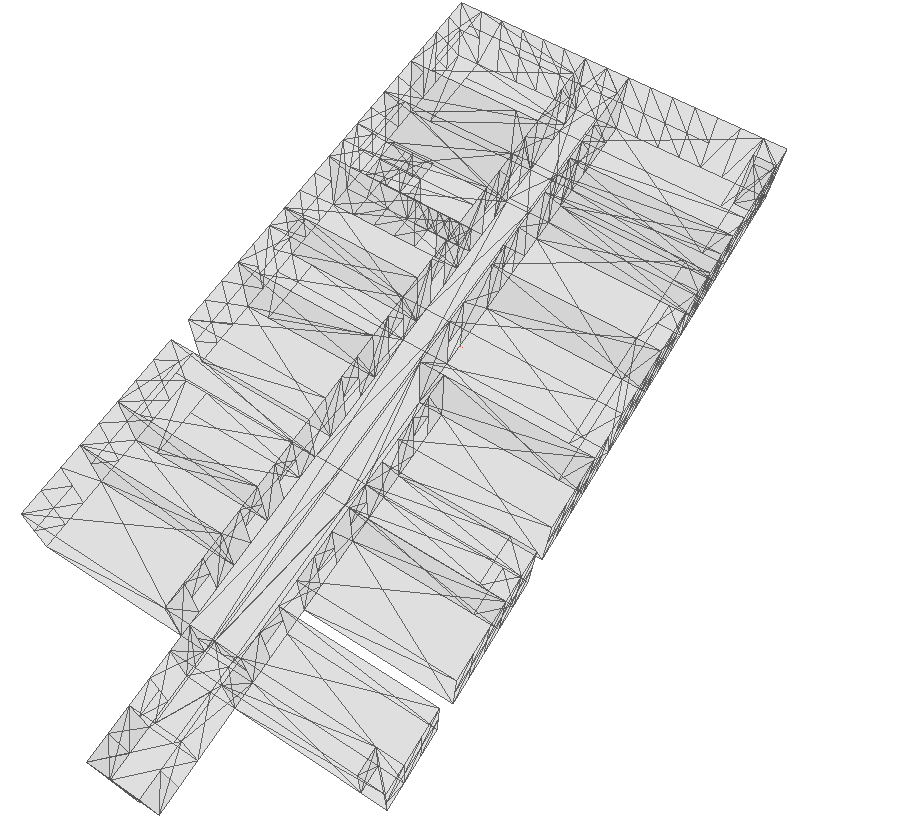
\includegraphics[width=\columnwidth]{pics/officemap}
\caption[Example polygon mesh]{An example polygon mesh of an office corridor at the Institute of Computer Science.}%
\label{fig:examplemap}%
\end{figure}

\end{document}